\documentclass{article}
\usepackage{listings}
\usepackage[T1]{fontenc}
\usepackage{titlesec}
\usepackage{graphicx}
\usepackage{amsmath}
\usepackage{xcolor}
\usepackage{amssymb}
\usepackage{circuitikz}
\usepackage{trace}
%\usepackage{minted}
\titleformat{\section}  % which section command to format
  {\fontsize{10}{12}\bfseries} % format for whole line
  {\thesection} % how to show number
  {1em} % space between number and text
  {} % formatting for just the text
  [] % formatting for after the text
  \title{Logika Cyfrowa}
\author{Jakub Gałaszewski} 
\begin{document}
\maketitle
\section{Napisz kod w asemblerze RISC V odpowiadający poniższemu wyrażeniu (w języku C lub podobnym). Załóż, że g oraz h już znajdują się w rejestrach x6 i x7, oraz wynik f powinien znaleźć się w rejestrze x5.}
\begin{lstlisting}
f = g + h - 5;
\end{lstlisting}
\begin{lstlisting}
add x5, x6, x7
addi x5, x5, -5
\end{lstlisting}
\section{Napisz wyrażenie w języku C (lub podobnym) odpowiadające poniższym instrukcjom asemblera RISC V.}
\begin{lstlisting}
add x1, x2, x3
add x1, x4, x1
\end{lstlisting}
\begin{lstlisting}
ans = x + y + z;
\end{lstlisting}
\section{Tablice w języku C (oraz w wielu innych językach) są kodowane w pamięci przez zapisanie kolejnych elementów tablicy jeden po drugim, w kolejnych adresach. W tablicach indeksowanych od 0 (jak w języku C) adres elementu o indeksie 0 (czyli pierwszego elementu) jest tożsamy z adresem całej tablicy. Napisz kod w asemblerze RISC V odpowiadający poniższemu wyrażeniu. Załóż, że adresy tablic A i B, których elementy są pojedynczymi bajtami, znajdują się w rejestrach x10 oraz x11, natomiast wartości zmiennych i oraz j znajdują się w x28 i x29.}
\begin{lstlisting}
B[8] = A[i-j]
\end{lstlisting}
\begin{lstlisting}
sub x3, x28, x29
add x10, x10, x3
lw x1, 0(x10) 
sw x1, 8(x11)
\end{lstlisting}
\section{Napisz wyrażenie w języku C (lub podobnym), wykorzystujące tablice, odpowiadające poniższym instrukcjom asemblera RISC V.}
\begin{lstlisting}
lb x30, 8(x12)
add x30, x30, x5
add x31, x12, x6
sb x30, 0(x31)
\end{lstlisting}
\begin{lstlisting}
x = A[8]
x += i;
A[c] = x;

x12[x6]=x12[8]+x5
\end{lstlisting}
\section{Określ, jaka instrukcja jest zakodowana przez następujące wartości pól, oraz jaki jest jej kod binarny:}
\begin{lstlisting}
opcode=0x3, funct3=0x2, rs1=27, rd=3, imm=0x4
\end{lstlisting}
opcode to opkod równy 3, czyli to load.\\
funct3 to lw, load word (ze znakiem).\\
rd to register destination równy 3.\\
rs to register source równy 27.\\
imm to wartość 12-bitowej stałej lub offsetu równe 4.\\
mamy format I, czyli:\\
000000000100 11011 010 00011 0000011\\
a sama operacja to lw x3, 4(x27) 
\section{Zapisz w kodzie binarnym RISC V poniższą instrukcję}
\begin{lstlisting}
sw x5, 32(x30)
\end{lstlisting}
store korzystamy w formacie S
\begin{center}
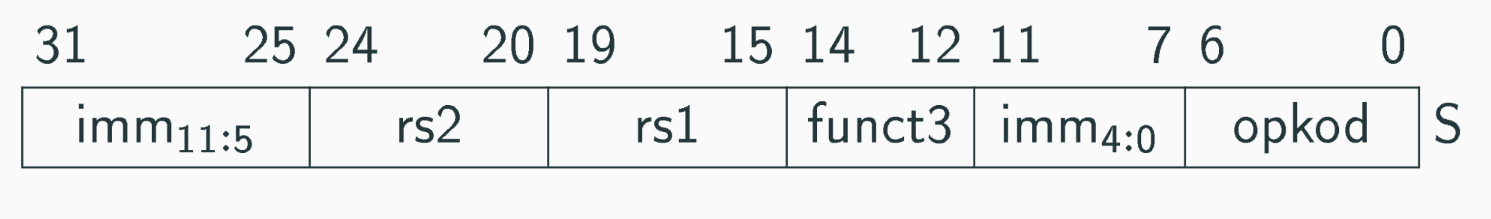
\includegraphics[scale=0.3]{./L12Z06.png}
\end{center}
pierwsze 7 bitów to starsze 7 bitów offsetu, 5 bitów to kolejno źródłowy adres i bazowy rejestr, funct koduje rodzaj dostęp pamięci, następnie mamy 5 bitów młodszych offsetu i na końcu opkod.\\
opkod to 0100011,\\ 
imm to 0000001 00000,\\
podobno funct3 to 010,\\ 
rs2 to 00101, \\
rs1 to 11110,\\
tak więc wynik to: 0000001 00101 11110 010 00000 0100011
\section{Jaka instrukcja jest zakodowana w kodzie binarnym RISC V poniżej?}
0000 0000 0001 0000 1000 0000 1011 0011\\
0000000 00001 00001 000 00001 0110011\\
funct3 to 000 funct7 to 0000000, czyli mamy add\\
rs2 to 1, rs1 to 1, rd to 1
czyli mamy 
\begin{lstlisting}
add x1, x1, x1
\end{lstlisting}
\section{Załóz, że w rejestrze x5 jest wartość 0x0000aaaa, zaś w rejestrze x6 jest wartość 0x12345678. Jaka jest wartość x7 po następujących operacjach?}
\begin{lstlisting}
a)  slli x7, x5, 4
	or x7, x7, x6
b)  srli x7, x5, 3
	andi x7, x7, 0xfef
a)	x7 = 0x000aaaa0
	x7 = 0x123EFEF8
b)	x7 = 0x00000aaa
	x7 = 0xffffffef
\end{lstlisting}
haczyk b jest taki, że 0xfef jest ze znakiem.
\section{Napisz w asemblerze RISC V procedurę obliczającą wartość liczby naturalnej zapisanej zapisanej w kodzie ASCII, w systemie dziesiętnym, w ciągu znaków zakończonym bajtem zerowym (jak w języku C). Parametr do procedury –  adres pierwszej litery ciągu znaków – będzie zapisany w rejestrze a0 (czyli x10), po zakończeniu działania procedury wynik również powinien się znaleźć w a0.}
\begin{lstlisting}
	 and t0, t0, x0
	 lbu t1, 0(a0)
loop:beq t1, x0, end
     slli t0, t0, 1
     slli t2, t0, 2
     add t0, t0, t2
     subi t1, t1, 48
     add t0, t1, t0
     addi t1, t1, 1
     j loop
end  mv a0, t0
	 ret

\end{lstlisting}
\end{document}
